\documentclass[
  12pt,       
  openright,      
  twoside,      
  a4paper,      
  english,      
  french,       
  spanish,      
  brazil,     
  ]{abntex2}
\usepackage{cmap}
\usepackage{lmodern}    
\usepackage[T1]{fontenc}
\usepackage[utf8]{inputenc} 
\usepackage{lastpage}   
\usepackage{indentfirst}               
\usepackage{color}        
\usepackage{graphicx}     
\usepackage{lipsum}     
\usepackage[brazilian,hyperpageref]{backref}  
\usepackage[alf]{abntex2cite}
\usepackage{listings}

\renewcommand{\lstlistingname}{Código}
\renewcommand{\lstlistlistingname}{Lista de códigos}

\begingroup\makeatletter
\let\newcounter\@gobble\let\setcounter\@gobbletwo
  \globaldefs\@ne \let\c@loldepth\@ne
  \newlistof{listings}{lol}{\lstlistlistingname}
  \newlistentry{lstlisting}{lol}{0}
\endgroup

\renewcommand{\cftlstlistingaftersnum}{\hfill--\hfill}

\let\oldlstlistoflistings\lstlistoflistings
\renewcommand{\lstlistoflistings}{%
   \begingroup%
   \let\oldnumberline\numberline%
   \renewcommand{\numberline}{\lstlistingname\space\oldnumberline}%
   \oldlstlistoflistings%
   \endgroup}

\lstdefinestyle{prologCustom}{
  alsoother={0123456789_},
  backgroundcolor=\color{white},
  basicstyle=\ttfamily\ABNTEXfontereduzida, 
  backgroundcolor=\color{white},
  breakatwhitespace=false, 
  breaklines=true,     
  captionpos=b,       
  commentstyle=\color{green},  
  deletekeywords={...},      
  escapeinside={\%*}{*)},          
  extendedchars=true,      
  frame=single,                   
  inputencoding=utf8,
  keepspaces=true,               
  keywordstyle=\color{blue},       
  literate={á}{{\'a}}1 {ã}{{\~a}}1 {é}{{\'e}}1 {è}{{\`{e}}}1 {ê}{{\^{e}}}1 {ë}{{\¨{e}}}1 {É}{{\'{E}}}1 {Ê}{{\^{E}}}1 {û}{{\^{u}}}1 {ú}{{\'{u}}}1 {â}{{\^{a}}}1 {à}{{\`{a}}}1 {á}{{\'{a}}}1 {ã}{{\~{a}}}1 {Á}{{\'{A}}}1 {Â}{{\^{A}}}1 {Ã}{{\~{A}}}1 {ç}{{\c{c}}}1 {Ç}{{\c{C}}}1 {õ}{{\~{o}}}1 {ó}{{\'{o}}}1 {ô}{{\^{o}}}1 {Õ}{{\~{O}}}1 {Ó}{{\'{O}}}1 {Ô}{{\^{O}}}1 {î}{{\^{i}}}1 {Î}{{\^{I}}}1 {í}{{\'{i}}}1 {Í}{{\~{Í}}}1,
  morekeywords={*, :-},
  numberbychapter=false,
  numbers=left,                    
  numbersep=5pt,                  
  numberstyle=\tiny\color{black}\sffamily, 
  rulecolor=\color{black},         
  showspaces=false,                
  showstringspaces=false,         
  showtabs=false,                  
  stepnumber=4,                    
  stringstyle=\color{blue}\itshape,     
  tabsize=2,                      
  title=\lstname,                 
  framexleftmargin=10pt,
  framexleftmargin=15pt
}
\lstset{style=prologCustom}

\renewcommand{\backrefpagesname}{Citado na(s) página(s):~}
\renewcommand{\backref}{}
\renewcommand*{\backrefalt}[4]{
  \ifcase #1
    Nenhuma citação no texto.
  \or
    Citado na página #2.
  \else
    Citado #1 vezes nas páginas #2.
  \fi}

\titulo{Sintetizador de voz para a avaliação da qualidade da voz disfônica}
\autor{Lucas Moura Veloso}
\local{Belo Horizonte}
\data{Junho de 2017}
\orientador{Prof. Dr. Maurílio Nunes Vieira}
\instituicao{
  Universidade Federal de Minas Gerais -- UFMG
  \par
  Escola de Engenharia
  \par
  Curso de Graduação em Engenharia Elétrica}
\tipotrabalho{Trabalho de Conclusão de Curso}

\preambulo{Monografia apresentada durante o Seminário dos Trabalhos de Conclusão do Curso de Graduação em Engenharia Elétrica da UFMG, como parte dos requisitos necessários à obtenção do título de Engenheiro Eletricista. A área de concentração é a de processamento digital de voz.}

\definecolor{blue}{RGB}{41,5,195}
\makeatletter
\hypersetup{
      %pagebackref=true,
    pdftitle={\@title}, 
    pdfauthor={\@author},
      pdfsubject={\imprimirpreambulo},
      pdfcreator={LaTeX with abnTeX2},
    pdfkeywords={abnt}{latex}{abntex}{abntex2}{trabalho acadêmico}, 
    colorlinks=true,       
      linkcolor=blue,                   
      citecolor=blue,      
      filecolor=magenta, 
    urlcolor=blue,
    bookmarksdepth=4
}
\makeatother
\setlength{\parindent}{1.3cm}
\setlength{\parskip}{0.2cm} 
\makeindex

\begin{document}
\frenchspacing 
\pretextual

\imprimircapa
\imprimirfolhaderosto

\begin{dedicatoria}
   \vspace*{\fill}
   \centering
   \noindent
   \textit{Este trabalho é dedicado a todas as pessoas que em algum momento pensaram que não eram boas o suficiente para serem quem queriam.} \vspace*{\fill}
\end{dedicatoria}

\begin{agradecimentos}
Primeiramente, gostaria de agradecer à minha família e amigos, que me aguentaram durante essa época particularmente estressante da minha vida, não teria conseguido terminar sem o apoio de vocês. Kenia, Léo, Carolina, Camila, Marinalva, Guido, Thaís, Cris, Matheus, Sanja, Afonso, Carol, Wagner, Thays e mais um monte de gente, há espaço limitado nessa página.

Gostaria de agradecer também ao meu orientador, Prof. Dr. Maurílio Nunes Vieira, que foi mais do que prestativo durante essa jornada e que me mostrou o caminho para essa área do conhecimento, que pouco tinha ouvido falar até então.

Outra pessoa que merece agradecimentos é o Prof. Dr. Hani Camille Yehia, que me apresentou esta área durante uma das suas disciplinas e que me ensinou a usar o LaTeX.
\end{agradecimentos}

\begin{epigrafe}
   \vspace*{\fill}
  \begin{flushright}
    \textit{``There's nothing that can't be done, if we raise our voice as one.''\\
    (Michael Jackson, We've had enough)}
  \end{flushright}
\end{epigrafe}

\setlength{\absparsep}{18pt}
\begin{resumo}
Este trabalho trata do desenvolvimento de uma aplicação Python para profissionais de fonoaudiologia, com ferramentas de síntese de voz específicas para  a avaliação da qualidade de vozes disfônicas. A topologia do sintetizador utilizado neste trabalho é baseada no modelo fonte-filtro da produção da voz e na síntese por formantes.
 \textbf{Palavras-chaves}: síntese, voz, filtros, digitais.
\end{resumo}

\pdfbookmark[0]{\listfigurename}{lof}
\listoffigures*
\cleardoublepage

\pdfbookmark[0]{\listtablename}{lot}
\listoftables*
\cleardoublepage

\begin{simbolos}
  \item[$ F0 $] Frequência fundamental do pulso glótico
  \item[$ FG $] Frequência do pulso glótico
  \item[$ k $] Fator de assimetria do pulso glótico
  \item[$ AN $] Amplitude do formante nasal
  \item[$ A1 $] Amplitude do primeiro formante
  \item[$ FNP $] Frequência do polo nasal
  \item[$ BNP $] Largura de banda do polo nasal
  \item[$ BNZ $] Largura de banda do zero nasal
  \item[$ F1 $] Frequência do primeiro formante
  \item[$ B1 $] Largura de banda do primeiro formante
  \item[$ F2 $] Frequência do segundo formante
  \item[$ B2 $] Largura de banda do segundo formante
  \item[$ F3 $] Frequência do terceiro formante
  \item[$ B3 $] Largura de banda do terceiro formante
  \item[$ B4 $] Largura de banda do quarto formante
  \item[$ B5 $] Largura de banda do quinto formante
  \item[$ z $] Operador de deslocamento da transformada Z
  \item[$ BW $] Largura de banda
  \item[$ F $] Frequência de corte
  \item[$ T $] Período de amostragem
\end{simbolos}

\pdfbookmark[0]{\contentsname}{toc}
\tableofcontents*
\cleardoublepage

\textual

\chapter{Introdução}
Atualmente, o diagnóstico fonoaudiológico de distúrbios da voz é dado de forma subjetiva e requer extremo treinamento da audição do profissional e conta com a sua habilidade de discernimento de certas características da voz. O objetivo deste trabalho é criar uma ferramenta computacional que facilite este trabalho, sintetizando vozes programaticamente com perturbações que simulam os diversos tipos de vozes que um paciente poderia apresentar, reduzindo assim a quantidade de treinamento necessário e o elemento do erro humano.

Para isso será desenvolvido uma variação do sintetizador de formantes descrito \citeonline{klatt1980} com algumas mudanças baseadas na metodologia descrita em \citeonline{fant_g._1979} e em metodologias desenvolvidas pelo aluno e seu orientador, que permita não apenas uma síntese de voz, como também a adição de diversos tipos de controles e funcionalidades que simulem as diversas disfonias da voz, de forma similar aos resultados descritos em \citeonline{jorgelucero2014}.

Este trabalho está organizado da seguinte forma: 
\begin{alineas}
\item Introdução;
\item Revisão bibliográfica;
\item Teoria;
\item Metodologia;
\item Desenvolvimento e Resultados;
\item Trabalhos futuros;
\item Conclusão;
\item Bibliografia;
\item Apêndices.
\end{alineas}

\chapter{Revisão Bibliográfica}
\chapterprecis{Neste capítulo iremos discutir um pouco do histórico do problema, as soluções aceitas na literatura para o mesmo e o atual estado da arte.}
O sintetizador de formantes de \citeonline{klatt1980} foi escolhido para este problema devido à sua ampla aceitação e revisão no meio acadêmico, mas a síntese por formantes não é a única ferramenta que poderia ter sido escolhida. Nas subseções abaixo falaremos um pouco sobre os outros tipos de síntese de fala que poderiam ter sido utilizadas e finalmente sobre a ferramenta escolhida.

\section{História dos sintetizadores de voz}
\label{subsec:historia}
Talvez a ideia mais antiga de síntese de voz seja a síntese por articulação, sendo que suas origens podem ser rastreadas para os séculos 11 e 12. De forma muito arcaica estas máquinas são descritas como ``mechanical talking heads'', eram idealizadas como objetos físicos que simulavam os processos do trato vocal. Apesar de sua origem antiga, a primeira aparição na literatura científica formal destes aparelhos  se deu em \citeonline{tarnoczy1949speaking}.

No começo do século 20, os avanços na Engenharia Elétrica permitiram o desenvolvimento de sintetizadores de voz eletrônicos. O primeiro destes dispositivos a atingir um grande público foi o VODER, criado por Homer Dudley, porém este precisava de muito treinamento para ser utilizado, como explicado em \citeonline{hartmut_traunmuller_history}.

\begin{figure}
\centering
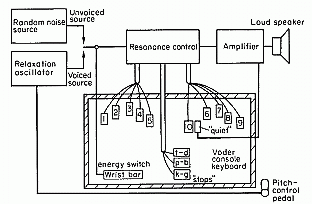
\includegraphics{imagens/voderdiagram.png}
\caption{Diagrama de funcionamento do VODER. Fonte: \citeonline{hartmut_traunmuller_history}.}
\label{fig:voderdiagram}
\centering
\end{figure}

\begin{figure}
\centering
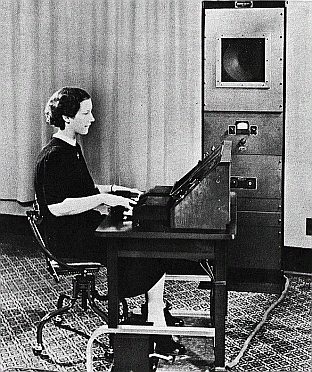
\includegraphics[scale=0.7]{imagens/voderuse.png}
\caption{Pessoa operando o VODER na \textit{World Fair} de Nova York em 1939. Fonte: \citeonline{hartmut_traunmuller_history}.}
\label{fig:voderuse}
\centering
\end{figure}

\begin{figure}
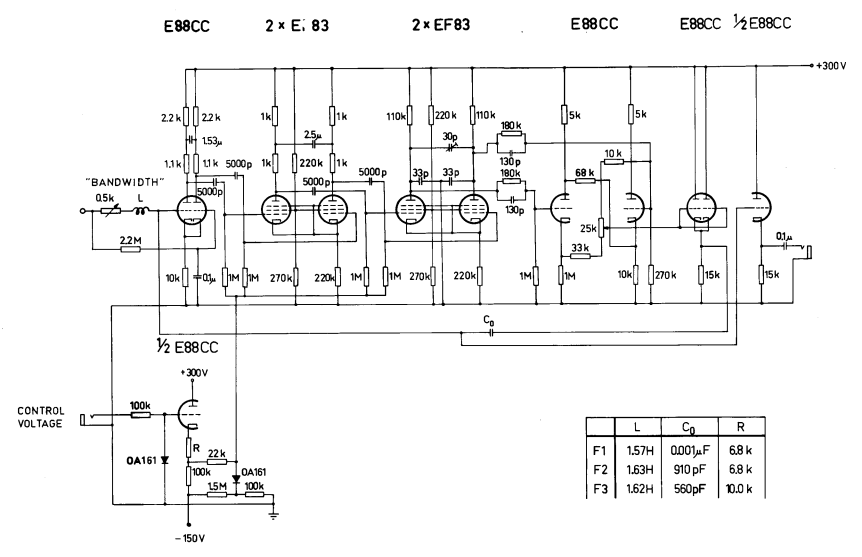
\includegraphics[width=\textwidth,keepaspectratio]{imagens/diagrama_polo_oveII.PNG}
\caption{Diagrama do circuito analógico para gerar os filtros ressoadores de formantes controlados por tensão do OVE II. Fonte: \citeonline{fant_g._speech}.}
\label{fig:oveIIdiagram}
\end{figure}

\begin{figure}
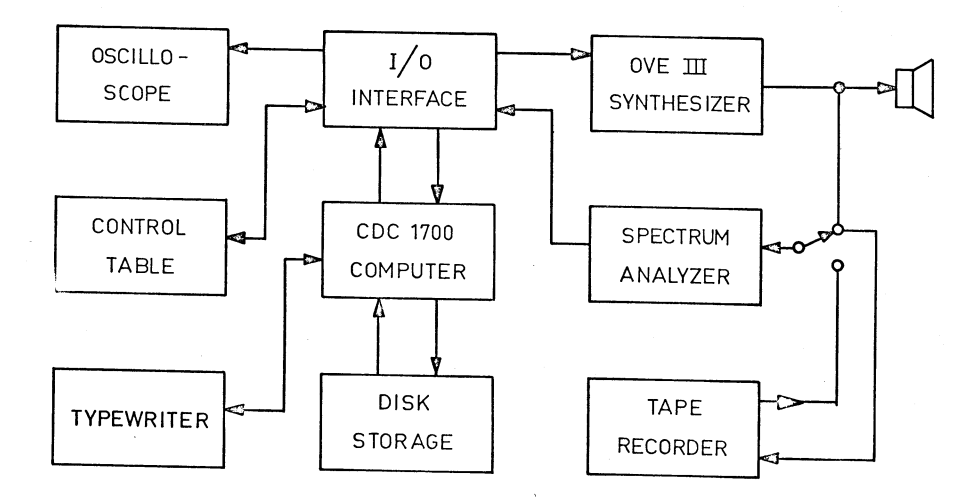
\includegraphics[width=\textwidth,keepaspectratio]{imagens/diagrama_geral_oveIII.PNG}
\caption{Diagrama geral do OVE III. Fonte: \citeonline{liljencrants_j._ove}.}
\label{fig:oveIIIdiagram}
\end{figure}

Durante os anos seguintes a área de sintese de voz continuou a crescer seguindo um caminho mais funcional e menos lúdico e baseado no entretenimento, foi então que começaram a surgir os sintetizadores analógicos que moldaram o caminho para o estado da arte atual. Como exemplo importante dos sintetizadores analógicos podemos destacar o OVE \cite{hartmut_traunmuller_history} e suas versões posteriores OVE II \cite{fant_g._speech} e OVE III \cite{liljencrants_j._ove} criados por Fant, G., Liljencrants, J. e a equipe do \textit{Royal Institute of Technology in Stockholm}.

Um aspecto interessante das versões do OVE desenvolvidas por Fant (I e II) é que eram totalmente analógicas e controladas manualmente, fazendo uso de circuitos analógicos para gerar e tratar os sinais de voz. Já o OVE III começou a usar circuitos digitais para algumas operações como uso básico de um teclado e uso de registradores e unidades de computação. As figuras \ref{fig:oveIIdiagram} e \ref{fig:oveIIIdiagram} demonstram um pouco do funcionamento destes modelos.

\section{Estado da arte}
\subsection{Síntese por articulação}
Esta técnica, descrita brevemente na seção \ref{subsec:historia}, atualmente é aplicável em software, com os mesmos conceitos de tentar emular os processos de formação de voz através de simulação dos processos físicos envolvidos.

\subsection{Síntese por concatenação}
Este método de síntese é baseada na junção de partes de áudios de fala para montar novas palavras. Existem vários tipo de implementações para esta arquitetura, porém a sua maior desvantagem é a necessidade de uma grande base de dados de amostras de fala e uma certa mecanicidade perceptível na fala devido aos cortes nos áudios, o que pode ser reduzido com o uso de algoritmos adequados de concatenação.

Uma implementação para este método pode ser encontrada em \citeonline{hunt1996unit} e um estudo sobre percepção humana e medidas objetivas foi realizado em \citeonline{stylianou2001perceptual}.

\subsection{Síntese por formantes}
A síntese por formantes não usa de áudios pré-gravados e nem tenta simular os processos físicos por trás da formação da fala, ao invés disso, o objetivo é gerar sinais e tratá-los com técnicas de processamento de sinais, de forma que o resultado final se aproxime o máximo possível da voz humana.

A sua base foi originalmente descrita em \citeonline{gold1968analysis} e sua implementação foi feita inicialmente em \citeonline{klatt1980}, onde descreve uma arquitetura de sintetizador que utiliza as formantes da voz e diversos outros parâmetros de controle para sintetizar vozes como vogais e fricativas. Esta configuração é amplamente aceita na comunidade acadêmica e já foi revisada extensamente, fazendo desta uma ótima plataforma para o desenvolvimento de um sintetizador de vozes disfônicas.

\subsection{Síntese de vozes disfônicas}
O campo de síntese de vozes disfônicas não trata de uma arquitetura de sintetizador e nem de técnicas para os mesmos, mas sim de uma visão mais geral da síntese digital de voz, que leva em consideração as disfunções do trato vocal que uma pessoa pode ter e sua síntese, gerando assim uma voz que se aproxime mais da real do locutor.

Atualmente esta é uma área muito estudada, alguns trabalhos que podem ser citados como referência do atual estado da arte nacional são \citeonline{jorgelucero2014}, que descreve um sintetizador digital por articulação de vozes disfônicas, e \citeonline{vieira2014measurement} que neste trabalho mediram o ruído glotal de vozes humanas e sintéticas por meio de algoritmos de processamento de imagens 2D.

\chapter{Teoria}
\label{sec:teoria}
\chapterprecis{Neste capítulo descreveveremos a teoria por trás da síntese por formantes para entendimento do trabalho. Maiores informações podem ser encontradas em \citeonline{klatt1980}.}
\section{Modelo fonte-filtro da produção da voz}
\label{subsec:fonteFiltro}
O modelo fonte-filtro da produção da voz, do modo como foi utilizado neste trabalho, basicamente visa emular o comportamento da laringe, faringe e das cavidades oral e nasal ao emitir sons, a partir de técnicas de processamento de sinais.

\begin{figure}
\centering
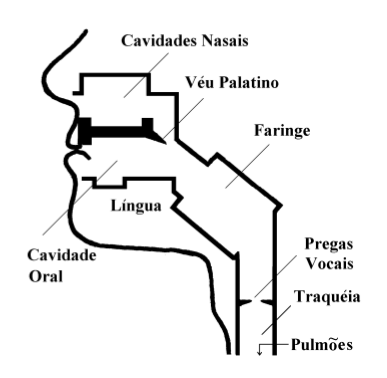
\includegraphics[scale=0.6]{imagens/trato_vocal.PNG}
\caption{Diagrama esquemático do trato vocal. Fonte: \citeonline{maurilio_1999}.}
\label{fig:tratoVocal}
\centering
\end{figure}

O pulmão gera um fluxo de ar, que ao passar pelas pregas vocais e em seguida pelas cavidades oral e nasal, são refinados e modulados, gerando assim a voz humana como conhecemos. A figura \ref{fig:geracaoPulsosGloticos} mostra o processo de abertura e fechamento da glote e como esta manipula o fluxo de ar que vem dos pulmões e gera os pulsos necessários para a vocalização. As cavidades do trato vocal, juntamente com a movimentação dos seus músculos, são os elementos de interesse deste modelo.

\begin{figure}
\centering
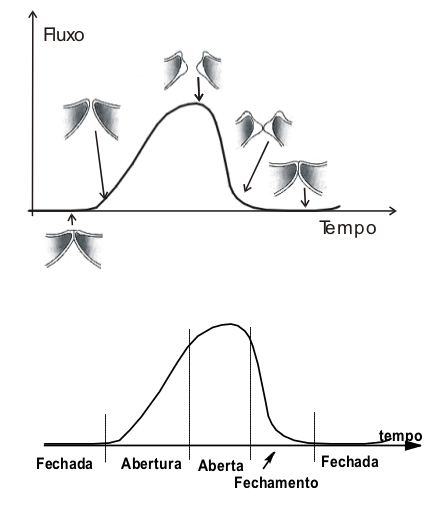
\includegraphics[scale=0.7]{imagens/geracao_pulso_glotico.PNG}
\caption{Diagrama de como a glote manipula o fluxo de ar para gerar os pulsos necessários para a vocalização. Fonte: \citeonline{maurilio_2004}.}
\label{fig:geracaoPulsosGloticos}
\centering
\end{figure}

As fontes do modelo são equivalentes aos pulsos gerados, como demonstrado na figura \ref{fig:geracaoPulsosGloticos}, enquanto os filtros são relacionados com os formantes e as características de radiação da onda sonora ao sair da cavidade oral, que se comporta como um filtro passa-altas. A figura \ref{fig:modeloFonteFiltro} mostra basicamente como a modelagem é feita.

\begin{figure}
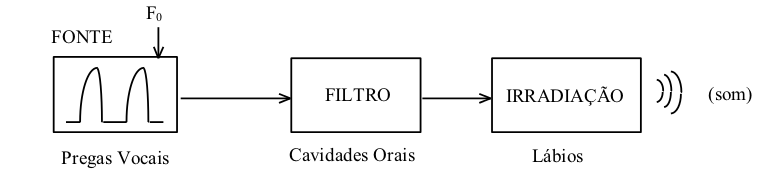
\includegraphics[width=\textwidth,keepaspectratio]{imagens/modelo_fonte_filtro.PNG}
\caption{Diagrama esquemático básico do modelo fonte-filtro da produção da voz. Fonte: \citeonline{maurilio_1999}.}
\label{fig:modeloFonteFiltro}
\end{figure}

Os formantes são regiões de alta energia do espectro sonoro e a intenção dos filtros é selecionar as frequências da onda gerada pelo pulso glótico para simular estas regiões de energia elevada. Segundo \citeonline{maurilio_1999}, as ordens dos formantes são relevante para síntese da voz da seguinte maneira:

\begin{citacao}
Os três primeiros formantes (F1, F2, F3) estão associados com o tipo de vogal, enquanto os formantes de ordem superior estão mais relacionados com a identidade vocal do locutor. \cite{maurilio_1999}.
\end{citacao}

O filtro de irradiação, ou radiação, figura \ref{fig:modeloFonteFiltro}, modela o comportamento da onda sonora ao sair do ambiente pressurizado da cavidade bucal e para o ambiente externo. Este pode ser implementado de diversas formas e será discutido com maior ênfase na seção \ref{subsec:teoriafiltros}.

\section{Teoria geral do sintetizador por formantes}
\label{subsec:teoriaSintetizador}
A figura \ref{fig:blockDiagram} abaixo nos mostra o diagrama de blocos utilizado para  geração do sinal de voz. A primeira etapa da síntese é a geração dos sinais de base, sendo estes uma série de pulsos com frequência igual à frequência fundamental escolhida para a fala e uma série aleatória para representar o ruído branco, que será tratado e adicionado para gerar os fricativos da voz.

\begin{figure}
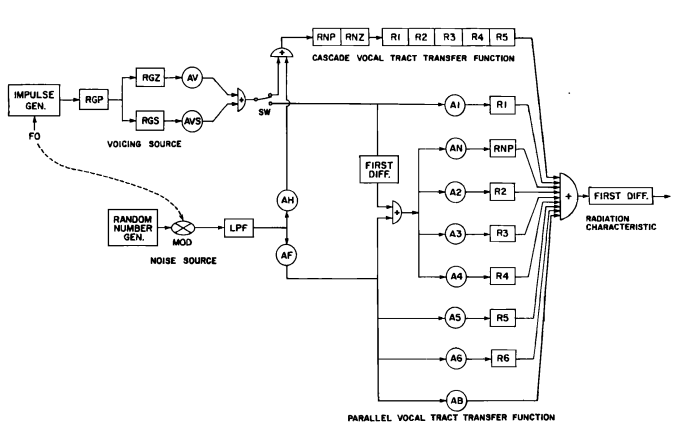
\includegraphics[width=\textwidth,keepaspectratio]{topografia_do_sintetizador}
\caption{Diagrama de blocos do sintetizador de formantes. Fonte: \citeonline{klatt1980}.}
\label{fig:blockDiagram}
\end{figure}

Os blocos $ Ri, 1 \leq i \leq 5 $ são filtros passafaixas ressonantes, que, quando parametrizados corretamente, modelam a série de pulsos com frequência fundamental F0 de forma a obter uma forma de onda semelhante aos pulsos glóticos da voz humana. A figura \ref{fig:glotalPulse} mostra a forma de onda obtida ao aplicarmos a metodologia de geração de pulsos glóticos descrita em \citeonline{klatt1980}.

\begin{figure}
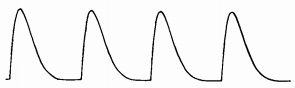
\includegraphics{pulso_glotal}
\centering
\caption{Forma de onda obtida usando a metodologia de \citeonline{klatt1980} para o pulso glotal. Fonte: \citeonline{klatt1980}.}
\label{fig:glotalPulse}
\centering
\end{figure}

A geração dos sinais pode se dar duas formas com o sintetizador de formantes, com a topologia em cascata ou em paralelo. Para este trabalho a implementação escolhida foi a em cascata por ser de implementação mais simples e de manutenção mais fácil, já que elimina a necessidade de ajustar os ganhos dos filtros separadamente.

A abordagem descrita em \citeonline{klatt1980} para geração de pulsos glóticos não é a mais adequada para este trabalho, pois existe uma falha básica na sua premissa que é o seu espelhamento no eixo do tempo quando comparado com pulsos reais (ver figuras \ref{fig:geracaoPulsosGloticos} e \ref{fig:glotalPulse}), além de fornecer pouca capacidade de customização da forma de onda a ser formada. Por estes motivos foi escolhida a abordagem descrita em \citeonline{fant_g._1979}, onde o pulso glótico é gerado numericamente, baseado na frequência fundamental F0, a frequência do pulso glótico FG e uma constante k que define a descida do pulso.

\begin{figure}
\centering
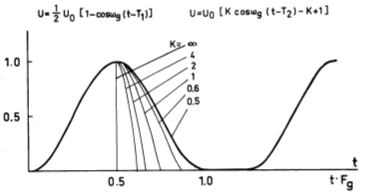
\includegraphics{imagens/pulso_glotico_fant_1979}
\caption{Modelo de geração dos pulsos glóticos. Fonte: \citeonline{fant_g._1979}.}
\label{fig:geracaoPulsosFant}
\centering
\end{figure}

O sistema foi desenvolvido de forma inteiramente digital mas poderia ser desenvolvido por filtros analógicos conhecidos e estudados durante o curso de Engenharia Elétrica, aplicando o diagrama acima  em um sistema analógico, de forma similar aos implementados em  \citeonline{fant_g._speech} e \citeonline{liljencrants_j._ove}.

Neste trabalho, o objetivo é que o sintetizador consiga gerar a vogal /a/. Para conseguir isto, os parâmetros utilizados foram calibrados de acordo com os valores descritos em \citeonline{klatt1980}, que foram obtidos de vozes reais e trazem maior verossimilhança para este trabalho.

\section{Filtros digitais ressonantes e antirressonantes}
\label{subsec:teoriafiltros}
Este trabalho faz uso de diversos tipos de filtros digitais, portanto a teoria por trás destes será brevemente explicada.

\begin{figure}
\centering
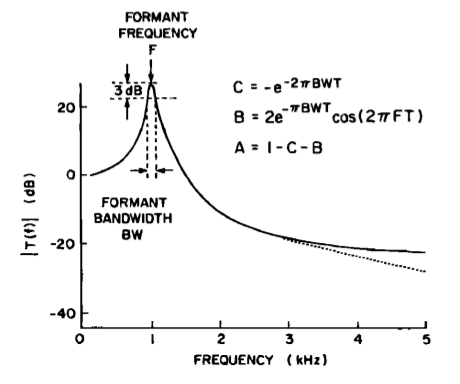
\includegraphics[scale=0.8]{imagens/grafico_filtro_digital.PNG}
\caption{Resposta em frequência de um filtro digital ressonante de formantes. Fonte: \citeonline{klatt1980}.}
\label{fig:respFreqFiltroDigital}
\centering
\end{figure}

Filtros ressonantes possuem uma característica em especial que os separam dos demais. Sua resposta frequência é de tal forma que a frequência de corte e a largura de banda formam uma faixa estreita que filtra qualquer frequência que não seja muito próxima da frequência de corte, que no caso deste trabalho é a frequência da formante. Um filtro deste tipo é exemplificado na figura \ref{fig:respFreqFiltroDigital}.

Estes filtros podem ser implementados das mais diversas formas e com várias tecnologias, porém utilizaremos apenas suas versões digitais, devido à natureza da implementação do projeto. De acordo com a metodologia descrita em \citeonline{klatt1980}, temos duas formas de desenvolver estes filtros, uma sequencial e baseada em iterações sobre blocos, ver figura \ref{fig:diagramaBlocoFiltroDigital}, e uma implementação voltada para a função de transferência do geral do filtro ressonante de formantes, que foi a elegida para ser utilizada. Esta equação no domínio da transformada Z é dada por:
\begin{equation}
\label{eq:filtroRessonante}
FiltroFormante(z) = \frac{A}{1 - Bz^{-1} - Cz^{-2} }
\end{equation}

O operador de deslocamento é dado pela variável z e os parâmetros A, B e C dependem de características da voz que queremos sintetizar, como pode ser visto nas equações \ref{eq:parametroA}, \ref{eq:parametroB} e \ref{eq:parametroC}, respectivamente.

\begin{equation}
\label{eq:parametroA}
A = 1 - C - B 
\end{equation}
\begin{equation}
\label{eq:parametroB}
B = 2e^{-\pi \cdot BW \cdot T}\cos(2\pi \cdot F \cdot T)
\end{equation}
\begin{equation}
\label{eq:parametroC}
C = -e^{-2\pi \cdot BW \cdot T}
\end{equation}

Os parâmetros BW, F e T das equações \ref{eq:parametroB} e \ref{eq:parametroC} representam, respectivamente, a largura de banda desejada para o filtro, a frequência de corte desejada e o período de amostragem utilizado.

O filtro antirressonante rejeitafaixa que modela o comportamento da cavidade nasal é basicamente o oposto de um filtro ressonante, sendo que sua resposta em frequência é o oposto da de um filtro ressonante baseado nos mesmos parâmetros, sua implementação neste trabalho é dada pela seguinte equação, também no domínio da transformada Z:
\begin{equation}
\label{eq:filtroAntiRessonante}
FiltroAntiRessonante(z) = \frac{A'z^{2} + B'z^{1} + C'z}{z^{2}}
\end{equation}

Onde os parâmetros A', B' e C' se baseiam nos parâmetros do filtro ressonante original das seguintes formas: 
\begin{equation}
\label{eq:antiA}
A' = \frac{1}{A}
\end{equation}
\begin{equation}
\label{eq:antiB}
B' = \frac{-B}{A}
\end{equation}
\begin{equation}
\label{eq:antiC}
C' = -C \cdot A
\end{equation}

\begin{figure}
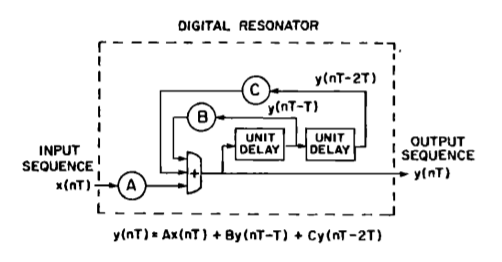
\includegraphics[width=\textwidth,keepaspectratio]{imagens/diagrama_bloco_filtro_digital.PNG}
\caption{Diagrama de blocos de um filtro digital ressonante. Fonte: \citeonline{klatt1980}.}
\label{fig:diagramaBlocoFiltroDigital}
\end{figure}

Os filtros utilizados tem as seguintes funções:
\begin{alineas}
\item Nasal
\item Formante 1
\item Formante 2
\item Formante 3
\item Formante 4
\item Formante 5
\item Radiação
\end{alineas}

O filtro nasal, indicado pelos blocos RNP e RNZ na figura \ref{fig:blockDiagram} nos dão uma aproximação da nasalização das vogais e de murmúrios nasais da voz, ambos formam um par de filtros digitais ressonantes e antirressonantes.

Os filtros de formantes simulam os formantes presentes na voz e os seus parâmetros foram calculados com base nos dados contidos em \citeonline{klatt1980}.

O filtro de radiação o efeito da radiação da onda sonora ao sair da boca do indivíduo falante e é basicamente um filtro digital passa-altas. Sua equação no domínio da transformada Z é dada por:
\begin{equation}
\label{eq:filtroRadiacao}
FiltroRadiacao = \frac{z - 1}{z}
\end{equation}

\chapter{Metodologia}
\chapterprecis{Este capítulo tratará dos métodos, tecnologias e técnicas que serão utilizadas no desenvolvimento do sintetizador.}
\section{Escolha das tecnologias}
Para o desenvolvimento do protótipo inicial do sintetizador, foi utilizado o ambiente de desenvolvimento MATLAB \cite{matlab}, devido à sua facilidade de uso e sua ampla e confiável biblioteca de processamento de sinais e de geração de áudios a partir de sinais digitais. Como o foco do trabalho era gerar um produto de software que pudesse ser utilizado para gerar amostras para terceiros, o MATLAB foi descartado como opção de desenvolvimento completo do projeto.

Para o produto final deste trabalho entretanto, a linguagem de programação escolhida foi Python 3.6, por ser de bom conhecimento do aluno, pela sua extensa documentação e por apresentar uma imensa possibilidade de expansão devido aos diversos módulos e bibliotecas existentes. Os códigos foram desenvolvidos na IDE PyCharm Community Edition \cite{pycharm}, que é de acesso gratuito.

Outra vantagem do Python que levou à sua escolha foi a facilidade montar interfaces gráficas e gerar aplicações \textit{standalone}. Para a interface gráfica deste projeto foi utilizada a \textit{framework} Tkinter, que está presente na maioria das instalações do interpretador do Python 3.6.

Como Python não possui suporte nativo a operações de processamento digital de sinais, foi utilizada a biblioteca externa SciPy \cite{scipy}, uma biblioteca muito conhecida e validada para Python \textit{open source}, voltada para operações matemáticas e científicas mas que também possui funcionalidades para geração de áudios e gráficos, combinando em apenas um pacote a maioria das funcionalidades utilizadas neste trabalho.

Para versionamento do código e para garantir a sua integridade ao longo de todo o desenvolvimento, foi utilizada a ferramenta GitHub \cite{github}. Essa escolha foi feita porque é um dos padrões atuais da indústria de desenvolvimento de software e devido à sua integração com diversas plataformas de desenvolvimento, incluindo a PyCharm \cite{pycharm} utilizada neste trabalho. Os códigos desenvolvidos estão disponíveis no Apêndice 1, seção \ref{sec:apendice1}, e também no repositório online acessível em <https://github.com/lucas-mv/klatt>.

\section{Padrões de projeto}
\label{subsec:padroesProjeto}
\subsection{Padrões de linguagem}
Com o objetivo de manter o código limpo, de fácil entendimento e manutenção, foi adotada a convenção de código do Python, onde as variáveis são escritas com \textit{camel case}, as funções e métodos são separados, quando necessário, pelo caractere \textit{underline} e as classes tem seus nomes escritos com \textit{pascal case}. Como Python é uma linguagem fortemente baseada na identação, esta foi seguida à risca, de modo a deixar o código o mais funcional e limpo possível.

O código foi escrito em português do Brasil em sua maioria, exceto pelas chamadas de bibliotecas externas e palavras chaves da linguagem escolhida. Esta decisão foi tomada para que o código seja de fácil entendimento para futuros trabalhos nacionais e também com o intuito de servir como exemplo deste tipo de trabalho para desenvolvedores brasileiros que queiram adentrar no mundo da síntese de voz por formantes.

\subsection{Estrutura do projeto}
O projeto foi desenvolvido pelos padrões da programação orientada a objetos, seguindo os seus quatro pilares básicos: abstração, encapsulamento, herança e polimorfismo. A escolha por este padrão foi feita para facilitar a reutilização de código, leitura e manutenção.

\begin{figure}
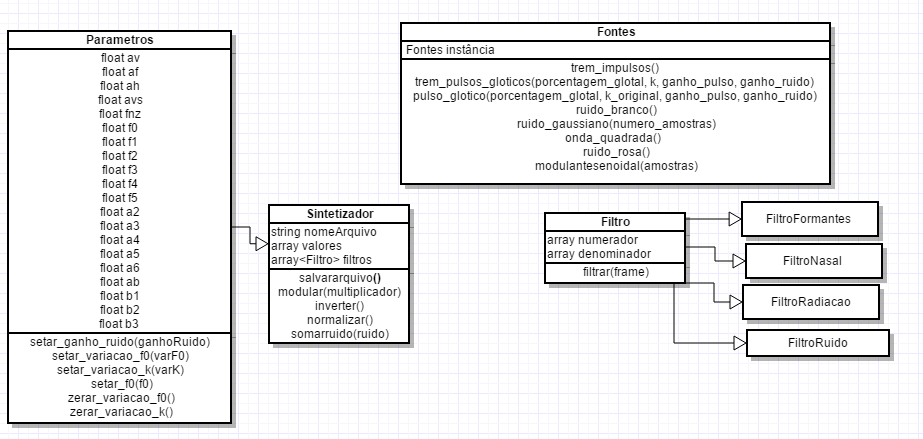
\includegraphics[width=\textwidth,keepaspectratio]{imagens/umlSintetizadorKlatt.PNG}
\caption{UML do relacionamento das classes do sintetizador desenvolvido, criada com a ferramenta online Gliffy \cite{gliffy}.}
\label{fig:umlsintetizador}
\end{figure}

Os objetos utilizados foram separados em classes, cada uma representando um dos aspectos do sintetizador, a figura \ref{fig:umlsintetizador} mostra como as classes relacionam entre si. Além disso, uma importante decisão de projeto foi a de criar duas classes de uso geral: \textit{utils} e \textit{constantes}. A primeira contém métodos e funções de uso geral ao longo do código e a segunda contém todas as constantes usadas durante o desenvolvimento, de modo a evitar futuros problemas com variáveis definidas em tempo de execução e facilitar a leitura e compreensão do trabalho.

A estrutura do código foi pensada para que, futuramente, outros módulos possam ser acoplados a este módulo principal, como será descrito no capítulo Trabalhos Futuros \ref{sec:trabalhosfuturos}.

\chapter{Desenvolvimento e Resultados}
\chapterprecis{Este capítulo tratará do desenvolvimento do projeto como um todo, desde a prototipagem com MATLAB até os resultados finais.}
\section{Protótipo}
O desenvolvimento foi iniciado com um protótipo em MATLAB, onde foi seguido à risca o algoritmo para implementação do sintetizador de Klatt e foi comprovada a possibilidade de criação de variações deste que cumprissem os objetivos do trabalho.

Como o objetivo deste protótipo era apenas a validação da teoria e da metodologia, os seus resultados foram pouco satisfatórios, gerando vozes que não se assemelham muito com a realidade, porém serviram como base para os desenvolvimentos futuros.

Após a validação da teoria, o desenvolvimento do trabalho em si foi iniciado, levando em consideração a metodologia descrita na seção \ref{subsec:padroesProjeto}.

\section{Desenvolvimento do projeto}
Muitas imagens a partir do \textit{software} desenvolvido estão presentes neste capítulo. Para facilitar o entendimento do leitor, a tabela \ref{tab:parametrosImagens} contém os valores dos parâmetros utilizados na geração destes resultados.

\begin{table}[htb]
\centering
\ABNTEXfontereduzida
\caption[Parâmetros de entrada do \textit{software} utilizados na geração das imagens]{Parâmetros de entrada do \textit{software} utilizados na geração das imagens.}
\label{tab:parametrosImagens}
\begin{tabular}{ccc}
  \toprule
  Parâmetro & Valor & Unidade \\
    \midrule \midrule
    F0 & 150 & Hz\\
    \midrule
    Tempo de simulação & 2 & s\\
    \midrule
    Período de amostragem & 0.0001 & s\\
    \midrule
    Variação de F0 & 5 & \%\\
    \midrule
    Variação de k & 50 & \%\\
    \midrule
    Ganho do ruído & 0.5 & Adimensional\\
    \midrule
    Ganho do pulso & 1.0 & Adimensional\\
    \midrule
    k & 1.0 & Adimensional\\
    \midrule
    AN & 0.0 & dB\\
    \midrule
    A1 & 0.0 & dB\\
    \midrule
    F1 & 620 & Hz\\
    \midrule
    F1 & 80 & Hz\\
    \midrule
    F2 & 1220 & Hz\\
    \midrule
    B2 & 50 & Hz\\
    \midrule
    F3 & 2550 & Hz\\
    \midrule
    B3 & 140 & Hz\\
    \midrule
    B4 & 250 & Hz\\
    \midrule
    B5 & 200 & Hz\\
    \midrule
    FNP & 250 & Hz\\
    \midrule
    BNP & 250 & Hz\\
    \midrule
    BNZ & 100 & Hz\\
    \bottomrule
\end{tabular}
{
  \fonte{Dados retirados de \citeonline{klatt1980} e gerados empíricamente pelos autores.}
  \nota{Os demais parâmetros não citados aqui podem ser facilmente encontrados em \citeonline[p.~976]{klatt1980}.}
}
\end{table}

\subsection{Criação do modelo do pulso}
O modelo para criação de pulsos glóticos descrito em \citeonline{klatt1980} foi implementado com sucesso e os resultados se aproximaram dos apresentados na figura \ref{fig:glotalPulse}, porém esta abordagem de geração dos pulsos a partir de filtros trouxe diversas complicações. A inserção de ruídos não estava sendo precisa o suficiente, já que esta depende da modulação em amplitude do ruído com a modulante sendo uma onda quadrada de frequência igual F0 (ver figura \ref{fig:blockDiagram} para maiores detalhes), ou seja, a inserção do ruído é baseada no ciclo de trabalho desta onda modulante e não no pulso em si. Outro problema que tivemos foi a falta de possibilidades de variações da forma de onda obtida com esta abordagem. O controle do período de fechamento do pulso glótico é complexo e este método basicamente apenas permite a seleção da frequência fundamental F0 de modo simples. A seção \ref{subsec:teoriaSintetizador} contém uma descrição mais profunda deste método e das suas imperfeições identificadas.

\begin{figure}
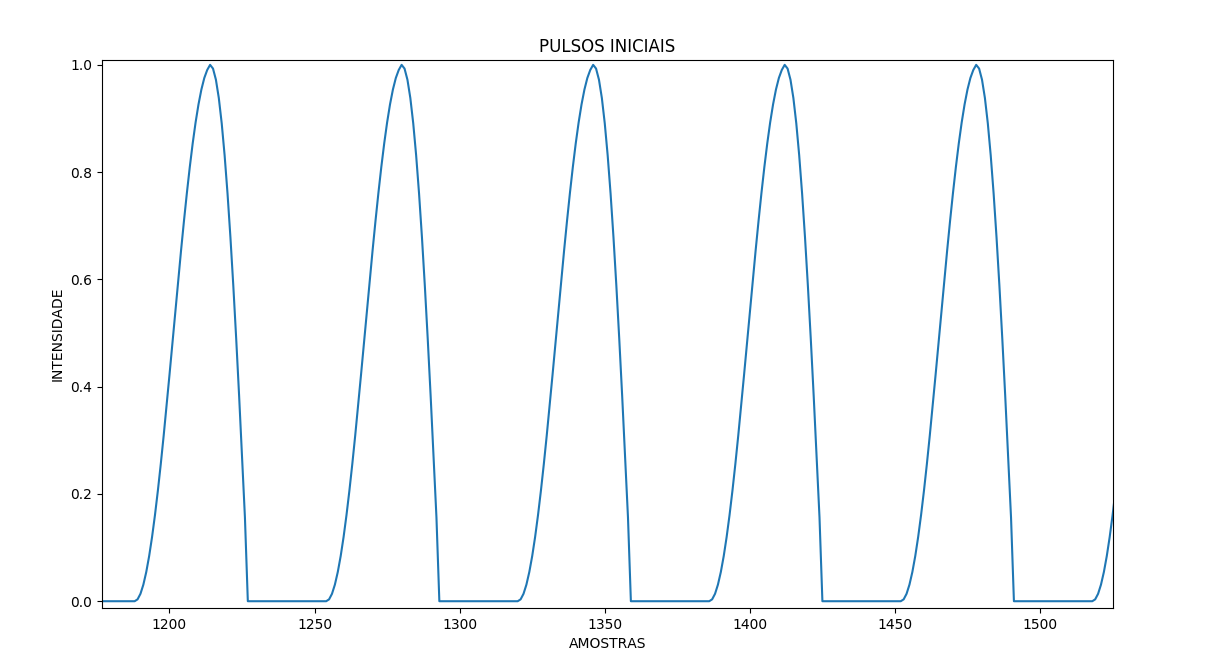
\includegraphics[width=\textwidth,keepaspectratio]{imagens/pulsos_iniciais_sem_variacoes.PNG}
\caption{Pulsos gerados com o algoritmo descrito em \citeonline{fant_g._1979}. Imagem gerada com o módulo Matplotlib, da biblioteca SciPy \cite{scipy}.}
\label{fig:pulsosSemVariacoes}
\end{figure}

Com isso, a abordagem foi modificada para gerar os pulsos segundo \citeonline{fant_g._1979}. Os resultados obtidos foram mais próximos de pulsos reais e podem ser analisados na figura \ref{fig:pulsosSemVariacoes}. Como citado anteriormente, desta forma temos controle maior dos tempos de silêncio e conseguimos configurar corretamente quando começam e terminam, possibilitando a inclusão de ruídos após o término do pulso, o que também se assemelha mais ao comportamento real.

Além disso, foi adicionado um controle de intensidade do pulso, podendo reduzir ou aumentar o seu valor final caso necessário. Para as amostras geradas neste trabalho e as inclusas na seção \ref{sec:apendice2}, foi utilizado o controle de pulsos em sua maior intensidade.

\subsection{Modelo e inserção do ruído}
Neste trabalho, o modelo do ruído utilizado tem distribuição gaussiana, como indicado em \citeonline{klatt1980}. Para gerar esta distribuição, foi utilizada o módulo Numpy da biblioteca SciPy \cite{scipy}, que possui além deste, diversos outros modelos de ruído, facilitando a sua troca caso este seja um parâmetro controlável futuramente.

Após o término de um pulso, as amostras de ruído são geradas e somadas aos valores iniciais durante o período de maior aproximação das pregas vocais, como pode ser visto na figura \ref{fig:pulsosComRuidos}. Este comportamento simula o real, já que, se neste período não houver o fechamento total das pregas vocais, haverá uma fenda que gerará ruído de fricção.

\begin{figure}
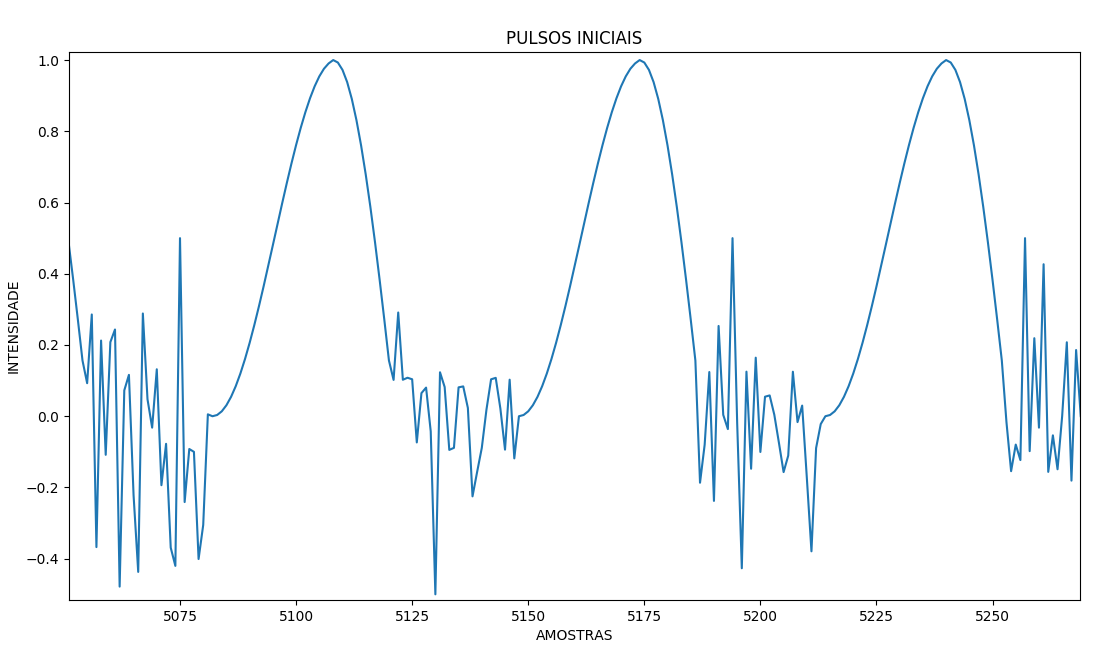
\includegraphics[width=\textwidth,keepaspectratio]{imagens/pulsos_iniciais_ft_ruido.PNG}
\caption{Pulsos gerados com adição dos ruídos. Imagem gerada com o módulo Matplotlib, da biblioteca SciPy \cite{scipy}.}
\label{fig:pulsosComRuidos}
\end{figure}

Foi adicionado um parâmetro de controle de intensidade do ruído, similar ao controle de intensidade dos pulsos, para possibilitar a geração de vozes pouco ou nada ruidosas, uma das premissas originais deste trabalho. Para gerar as figuras contidas aqui e as amostras da seção \ref{sec:apendice2}, este controle foi configurado como 50\% do valor máximo total. Devido à natureza do ruído gaussiano e de modo a garantir que este não ultrapasse o valor máximo dos pulsos e fique sempre contido neste intervalo, os valores gerados são normalizados entre 0\% e o valor de controle.

\subsection{Controle de variação de F0 e de k}
\begin{figure}
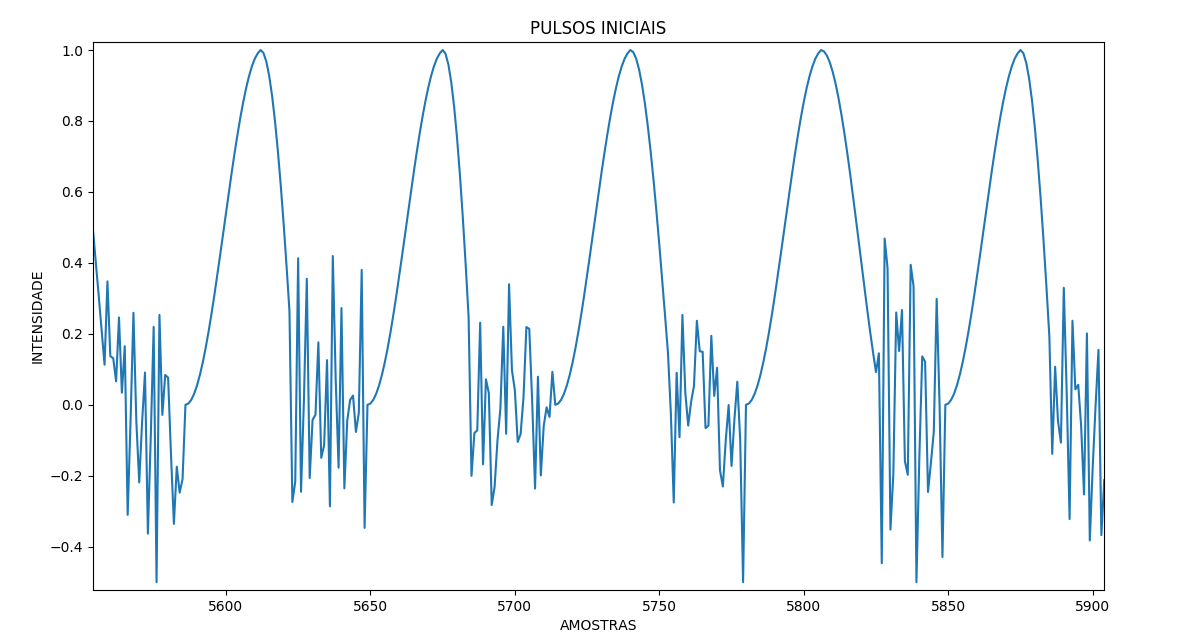
\includegraphics[width=\textwidth,keepaspectratio]{imagens/pulsos_ft_variacoes.PNG}
\caption{Pulsos com ruído adicionado e com variações sutis na frequência fundamental (F0) e na velociadade de descida (k). Imagem gerada com o módulo Matplotlib, da biblioteca SciPy \cite{scipy}.}
\label{fig:pulsosComVariacoes}
\end{figure}
Para melhorar a qualidade da voz sintetizada e também dar mais controle para o usuário final, foi gerada uma rotina de variação de F0 e de k pulso a pulso. Desta forma cada pulso será diferente do outro não somente no ruído como também em pequenas variações de frequência fundamental e de velocidade de queda. A figura \ref{fig:pulsosComVariacoes} mostra um pulso com estes controles de variação habilitados.

Para gerar as amostras contidas na seção \ref{sec:apendice2} e da figura \ref{fig:pulsosComVariacoes} os parâmetros foram configurados da seguinte forma:
\begin{equation}
VariaçãoPercentualF0 = 5\%
\end{equation}
\begin{equation}
VariaçãoPercentualK = 50\%
\end{equation}
Estes valores foram adequados ao longo de vários testes e apresentam uma variação factível destes parâmetros e que dão uma melhor sonoridade ao áudio gerado.

\subsection{Arquitetura dos filtros e filtragem dos sinais gerados}
Para a implementação dos filtros, foi usada a estrutura de herança descrita em detalhes na seção \ref{subsec:padroesProjeto} e o módulo \textit{signal} da biblioteca SciPy \cite{scipy}, bem como a teoria descrita em \ref{subsec:teoriafiltros}. Os parâmetros de cada um dos filtro podem ser facilmente modificados no sintetizador desenvolvido, alterando os dados de entrada da classe \textit{Parametros}, cuja estrutura também é explicada com mais detalhes na seção \ref{subsec:padroesProjeto}.

\begin{figure}
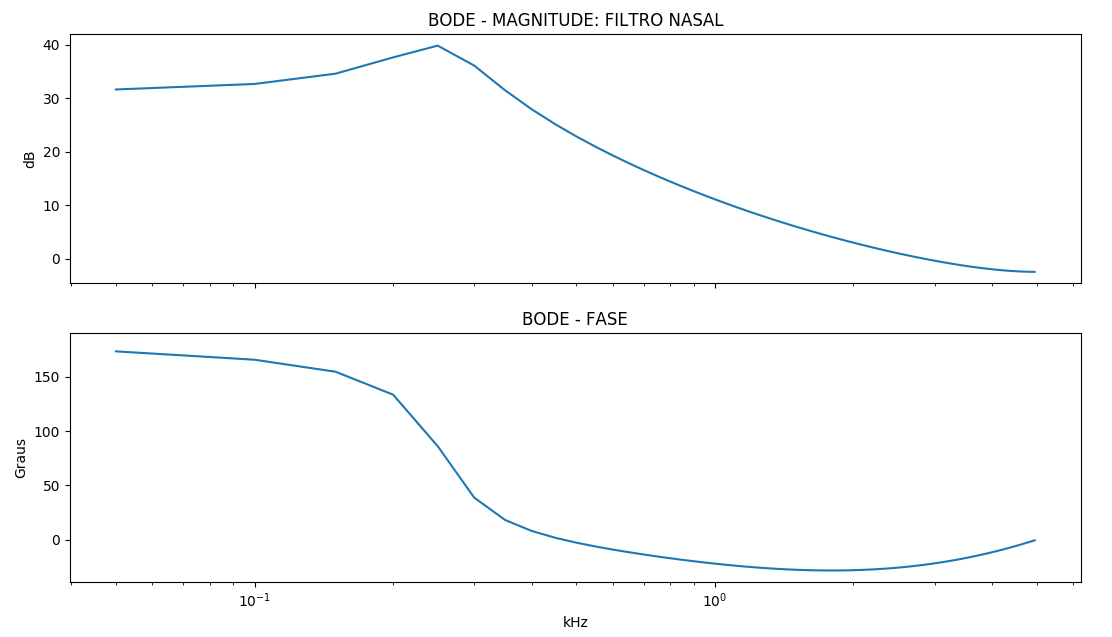
\includegraphics[width=\textwidth,keepaspectratio]{imagens/bode_nasal.PNG}
\caption{Diagrama de Bode do filtro que simula o comportamento nasal desenvolvido. Imagem gerada com o módulo Matplotlib, da biblioteca SciPy \cite{scipy}.}
\label{fig:filtroNasal}
\end{figure}

\begin{figure}
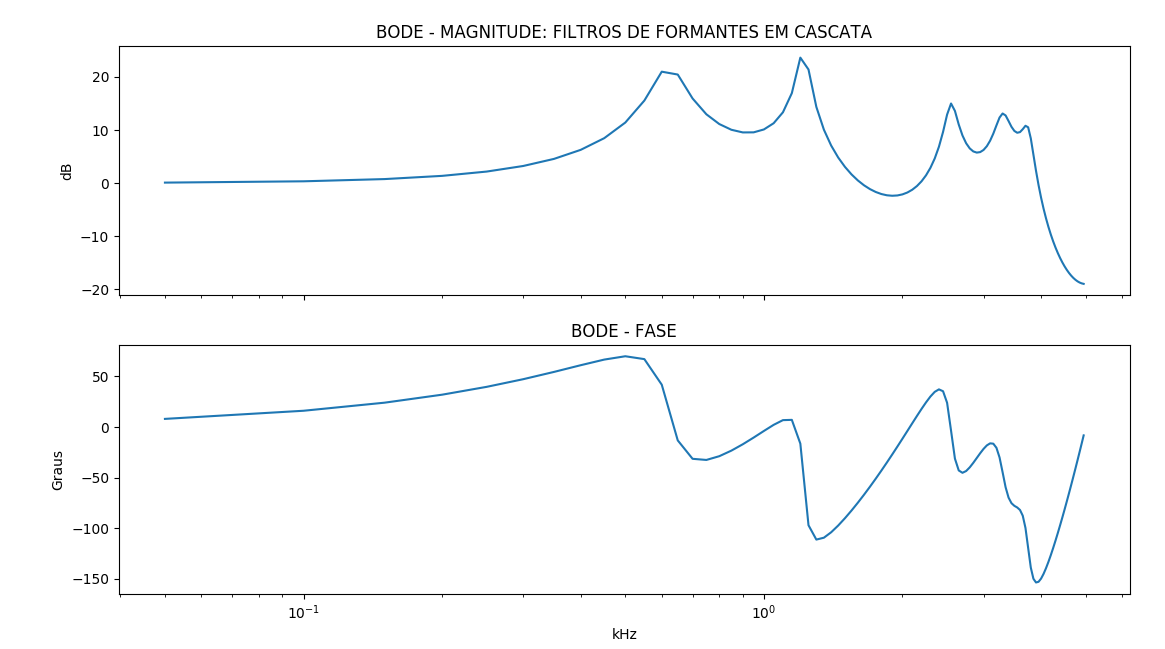
\includegraphics[width=\textwidth,keepaspectratio]{imagens/bode_formantes.PNG}
\caption{Diagrama de Bode do filtro de formantes desenvolvido, onde os formantes 1, 2, 3, 4 e 5 já estão em cascata. Imagem gerada com o módulo Matplotlib, da biblioteca SciPy \cite{scipy}.}
\label{fig:filtroFormantes}
\end{figure}

\begin{figure}
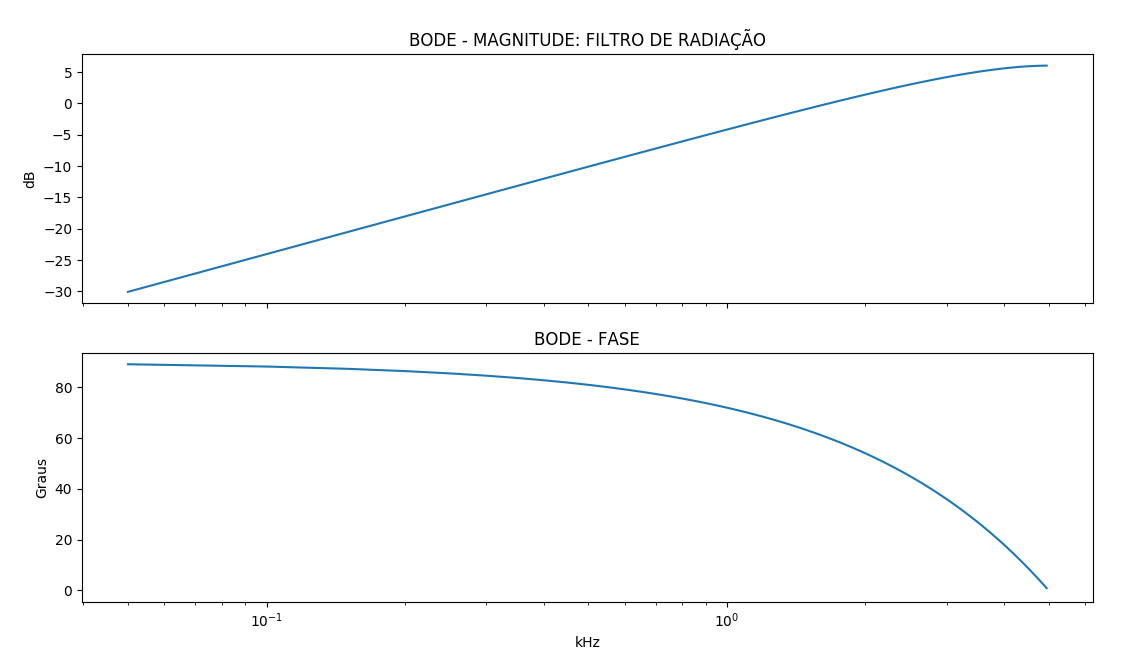
\includegraphics[width=\textwidth,keepaspectratio]{imagens/bode_radiacao.PNG}
\caption{Diagrama de Bode do filtro de radiação desenvolvido. Imagem gerada com o módulo Matplotlib, da biblioteca SciPy \cite{scipy}.}
\label{fig:filtroRadiacao}
\end{figure}

As figuras \ref{fig:filtroNasal}, \ref{fig:filtroFormantes} e \ref{fig:filtroRadiacao} mostram os diagramas de Bode dos filtros gerados. É importante salientar que os resultados da saída dos filtros serão normalizados para valores entre 0.0 e 1.0, fazendo com que o ganho destes filtros seja apenas uma forma de selecionar as frequências de interesse.

Seguindo o fluxo de operação do sintetizador, os pulsos serão gerados, adicionados de ruído e, em seguida, filtrados por estes em cascata, um após o outro.

\subsection{Geração do arquivo de áudio}
Após todos esses processos o arquivo de áudio é gerado e salvo com o nome dado pelo usuário no começo da execução do programa. Para gerar este arquivo foi utilizado o módulo \textit{wave} da biblioteca SciPy \cite{scipy}. A figura \ref{fig:ondaGerada} mostra uma forma de onda gerada por este sintetizador.

\begin{figure}
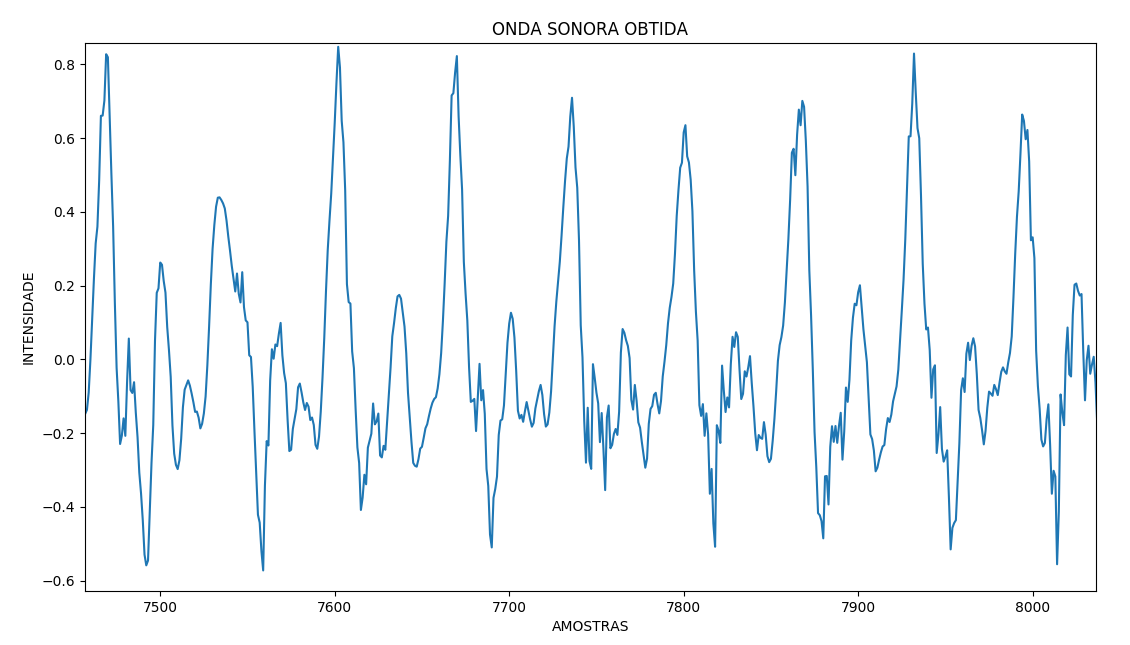
\includegraphics[width=\textwidth,keepaspectratio]{imagens/onda_gerada.PNG}
\caption{Parte da onda sonora final gerada pelo sintetizador. Imagem gerada com o módulo Matplotlib, da biblioteca SciPy \cite{scipy}.}
\label{fig:ondaGerada}
\end{figure}

\subsection{Interface gráfica}
Foi desenvolvida uma interface gráfica básica para usuários que desejam alterar alguns parâmetros do programa antes de sintetizar, que se mostrou bem útil para testar novas configurações e validar resultados. Foi desenvolvida com a \textit{framework} Tkinter, presente na maioria das versões do Python 3.6.

\begin{figure}
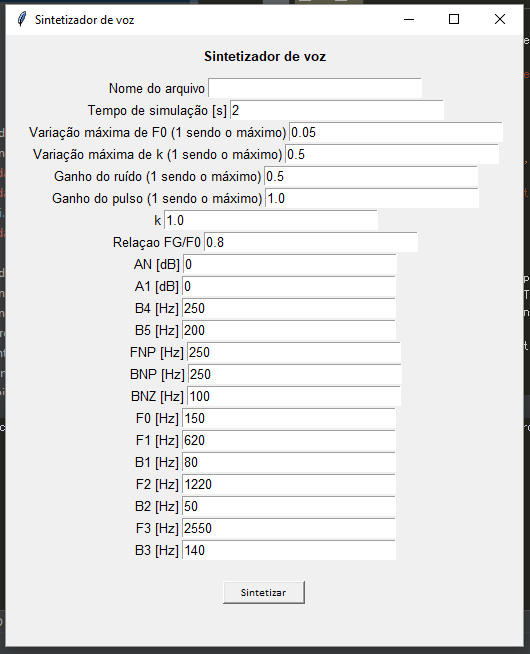
\includegraphics[width=\textwidth,keepaspectratio]{imagens/gui_basica.PNG}
\caption{Interface gráfica básica desenvolvida para o sistema, permite que o usuário altere alguns parâmetros antes de sintetizar a voz.}
\label{fig:guiBasica}
\end{figure}

Os parâmetros que o usuário pode modificar com esta interface são:
\begin{alineas}
\item Nome do arquivo
\item Tempo de simulação
\item Variação de F0
\item Variação de K
\item Ganho do ruído
\item Ganho do pulso
\item Relação FG/F0
\item K
\item AN
\item A1
\item B4
\item B5
\item FNP
\item BNP
\item BNZ
\item F0
\item F1
\item B1
\item F2
\item B2
\item F3
\item B3
\end{alineas}

Todos estes são parâmetros do sintetizador de Klatt, que estão explicados em sua totalizade em \citeonline{klatt1980} e \citeonline{fant_g._1979}, exceto pela ``Relação FG/F0'', que representa a porcentagem de F0 relativa à frequência do pulso glótico FG.

Ao clicar em no botão ``Sintetizar'' o \textit{software} tentará sintetizar a voz com os parâmetros inseridos e, ao terminar exibirá a mensagem ``Áudio sintetizado!'' abaixo do botão e salvará o arquivo na mesma pasta em que está o executável. Caso ocorra algum erro a mensagem exibida será ``Erro:'', seguida da descrição do erro.

\chapter{Trabalhos futuros}
\label{sec:trabalhosfuturos}
\chapterprecis{Este capítulo tratará das melhorias futuras que podem ser feitas, com relação a experiência do usuário, inclusão de funcionalidades e geração de conhecimento com este trabalho.}
\section{Experiência do usuário}
Vários módulos podem ser adicionados a este sintetizador para melhorar a experiência do usuário final, sendo os principais os seguintes:

\begin{alineas}
\item Melhoria da interface gráfica da aplicação \textit{standalone}
\item Criação de um sistema web e API para acessar o sintetizador
\item Criação de um aplicativo \textit{mobile} que execute as rotinas de sintetização
\end{alineas}

A seguir temos uma curta explicação de cada um destes itens e de como poderiam ser feitos.

\subsection{Melhoria da interface gráfica}
A \textit{framework} Tkinter permite a criação de interfaces gráficas muito mais complexas e responsivas do que a atual. Nada impediria de futuramente a GUI ser migrada para outra \textit{framework} que permita o desenvolvimento de um design melhor.

Melhorias possíveis de serem feitas e de complexidade não muito elevada seriam a melhor formatação da tela e o uso de entradas de dados mais amigáveis ao usuário, de modo a impedir que este cometa erros de entrada de parâmetros.

A seleção de caminho onde salvar o arquivo gerado e a inclusão de um menu de ajuda que explique cada um dos parâmetros também são melhorias muito interessantes para evitar frustrações ao operar o \textit{software}.

\subsection{Sistema web e API}
A criação de uma API que encapsula o módulo do sintetizador não seria muito complicado, existem muitas bibliotecas em Python voltadas para esta funcionalidade, a mais famosa atualmente sendo a \textit{framework} Django, acessível em <https://www.djangoproject.com>. Este pacote possui uma boa integração com a IDE PyCharm \cite{pycharm} utilizada para o desenvolvimento do projeto, facilitando ainda mais esta melhoria.

Esta API poderia ser acessada de diversas formas, um sistema web seria uma ótima opção já que os usuários teriam sempre uma versão atualizada do sistema ao acessar o sítio. Outra vantagem do sistema web são as inúmeras bibliotecas de desenvolvimento e de componentes visuais, bem como a facilidade de desenvolver designs amigáveis.

\subsection{Aplicativo}
Atualmente o desenvolvimento de aplicativos se tornou um processo bem simples e este poderia ser feito de diversas formas. Uma possibilidade seria a criação de uma API, assim como no item anterior, e criar um aplicativo que acesse esta. Outra possibilidade seria encapsular o módulo do sintetizador e gerar um aplicativo \textit{standalone} diretamente com este, utilizando alguma \textit{framework} de desenvolvimento \textit{mobile} própria do Python, como a Kivy, acessível em <https://kivy.org>.

Caso a abordagem da API seja escolhida, temos a possibilidade de desenvolvimento nativo para cada plataforma ou o uso de ferramentas multiplataformas, como Kony ou Xamarin, respectivamente acessíveis nos sítios <http://www.kony.com/pt> e <https://www.xamarin.com>.

\section{Funcionalidades futuras}
\label{subsec:funcionalidadesFuturas}
Importantes funcionalidades que podem ser implementadas futuramente são a geração de sonogramas das vozes sintetizadas e medições destas, principalmente da relação sinal-ruído (\textit{SNR}), da variação aleatória ciclo-a-ciclo da frequência fundamental F0 e da amplitude dos pulsos glóticos, respectivamente conhecidos como \textit{jitter} e \textit{shimmer}.

O sonograma poderia ser facilmente gerado com o módulo matplotlib da biblioteca SciPy \cite{scipy}, que já é usado neste projeto. As mudanças necessárias para incluir esta funcionalidade seriam pequenas e seria uma grande melhoria para usuários finais que usam esta ferramenta para avaliar a voz. A medição de SNR também pode ser feita com a biblioteca SciPy \cite{scipy}, usando módulo stats.

Outra abordagem seria, a partir do sonograma fazer as medições, seguindo o método descrito em \citeonline{vieira2014measurement}, que obteve resultados robustos, com diversos cenários diferentes, além de ter a vantagem de ser um método específico de medições em vozes disfônicas.

\section{Geração de conhecimento}
\label{subsec:geracaoConhecimento}
A síntese de vozes disfônicas é uma área em crescimento e este trabalho pode ser desenvolvido de diversas formas para acrescentar a esta.

Uma das formas que este trabalho pode contribuir com a área é fazendo testes de percepção com as diversas amostras geradas, contidas na seção \ref{sec:apendice2}. Estes testes nos mostrariam os limites da metodologia desenvolvida para gerar vozes similares às reais e dariam informações sobre onde é possível melhorar o algoritmo utilizado.

Os testes de percepção alinhados com as medições descritas na seção \ref{subsec:funcionalidadesFuturas} também forneceriam informações sobre os ganhos de qualidade e de customização da voz obtidos ao utilizar o método de gerar pulsos descrito em \citeonline{fant_g._1979} e os parâmetros de controle de ruído, intensidade dos pulsos, variação de k, F0 e da relação FG/F0.

Ainda sobre os testes de percepção, estes podem ser utilizados para avaliarmos a menor diferença perceptível com relação aos parâmetros envolvidos, trazendo assim melhor entendimento da relação destes com a qualidade da voz sintetizada. Tais estudos seriam importantes para que os usuários profissionais de fonoaudiologia tenham, nesta ferramenta, auxílio para quantificação de perturbações na voz associadas a alterações nas vibrações das pregas vocais.

Existe bastante possibilidade de melhoria do \textit{software} com relação à escolha dos parâmetros iniciais para a geração das vozes disfônicas, e é da vontade do desenvolvedor continuar este trabalho de modo a fazer uma compilação de parâmetros ideais para síntese de cada tipo de patologia da voz, porém isso só seria possível após os teste de percepção citados acima.

Outro estudo futuro que pode ser feito a partir deste trabalho é validar analiticamente, por meio das medições indicadas na seção \ref{subsec:funcionalidadesFuturas}, a existência dos fenômenos de \textit{jitter} e \textit{shimmer} nas vozes sintetizadas utilizando os controles de variação de F0 e k pulso a pulso. Tais fenômenos foram observados empiricamente durante o desenvolvimento do projeto, mas não houve tempo para realizar as medições necessárias e comprovar que a inserção destes controles foram as reais causas destes.

\chapter{Conclusão}
\chapterprecis{Este capítulo tratará das conclusões a serem tiradas deste trabalho, bem como das discussões que ocorreram ao longo do seu desenvolvimento.}
Várias conclusões podem ser tiradas sobre as diversos áreas deste trabalho, abaixo segue uma lista dos principais tópicos a serem abordados nessa seção:

\begin{alineas}
\item Desenvolvimento das habilidades profissionais e uso dos conhecimentos adquiridos no curso;
\item Qualidade do código;
\item Qualidade da voz sintetizada;
\item Melhorias observadas com o uso dos controles desenvolvidos;
\item Uso da metodologia descrita em \citeonline{fant_g._1979}.
\end{alineas}

\section{Desenvolvimento das habilidades profissionais}
Este trabalho sintetizou diversos conhecimentos adquiridos durante o curso, desde a parte de estruturação e organização do projeto até as habilidades de escrita de relatórios técnicos.

No início do desenvolvimento foi feito um estudo para chegar à estrutura descrita na seção \ref{subsec:padroesProjeto}, que só foi possível devido aos conhecimentos de estruturação de projetos em geral e mais especificamente de programação orientada a objetos, conhecimentos estes que foram adquiridos durante diversas matérias do curso de Engenharia Elétrica.

Muitas das técnicas de programação utilizadas neste projeto também foram aprendidas durante o curso, em especial nas disciplinas ``Programação Orientada a Objetos'' e ``Algoritmos e Estruturas de Dados II'', porém muitas foram adquiridas com a prática deste trabalho, principalmente as relacionadas à linguagem Python.

O uso de filtros digitais também foi essencial para o desenvolvimento do projeto, cuja compreensão só foi possível graças às disciplinas ``Processamento de Sinais'', ``Análise de Circuitos Elétricos II'', ``Análise de Circuitos Elétricos III'' e ``Análise de Sistemas Lineares''.

As habilidades de escrita de trabalhos acadêmicos, que foram muito utilizadas neste texto, também foram estudadas no curso, extensamente nas diversas disciplinas de laboratório, mas também nos projetos de pesquisa que foram desenvolvidos durante o tempo como graduando da UFMG.

\section{Qualidade do código}
Qualidade do código foi uma preocupação ao longo da evolução do projeto, visando manter a sua manutenção e compreensão sempre fácil tanto para o desenvolvedor quanto para terceiros que pudessem vir a analisá-lo posteriormente.

É da compreensão do autor que o código desenvolvido apresenta boa qualidade e respeita boas práticas da programação orientada a objetos e da linguagem escolhida, apesar de que sempre existem espaços para melhoria.

Houveram algumas mudanças na estrutura do código durante o desenvolvimento, porém nunca foram quebras explícitas da arquitetura do \textit{software} que dificultariam a manutenção do código.

\section{Qualidade da voz sintetizada}
O sintetizador desenvolvido conseguiu sintetizar corretamente vozes disfônicas com ruídos, os resultados foram bastante similares aos observados em pacientes com algumas patologias da voz.

Como grande parte do tempo gasto foi dedicado à implementação da teoria e da metodologia, ainda existe muita possibilidade de melhoria, principalmente na seleção dos parâmetros ideais para cada patologia da voz, como discutido na seção \ref{subsec:geracaoConhecimento}, e para cada perfil de pessoa falante.

\section{Controles adicionais desenvolvidos}
Com adição aos parâmetros já definidos em \citeonline{klatt1980} e em \citeonline{fant_g._1979}, foram desenvolvidos os controles adicionais de intensidade de ruído e do pulso, variação de F0 e de k e da relação FG/F0. Tais parâmetros foram inseridos para termos melhor controle sobre a voz a ser gerada.

Os resultados obtidos usando estes controles foram melhores do que os esperados, principalmente com relação à variação de F0 e de k. A variação de F0 pulso a pulso levou à geração de \textit{jitter} no áudio sintetizado, enquanto a variação de k gerou \textit{shimmer}, dois fenômenos presentes em vozes reais e que incorporaram verossimilhança ao produto final. Seria necessário fazer um estudo de medições destes fenômenos nas vozes sintetizadas para comprovar analiticamente a presença destes dois fenômenos, como descrito na seção \ref{subsec:geracaoConhecimento}.

O controle de intensidade do ruído se provou essencial para modular a voz de modo a simular a intensidade da patologia a ser sintetizada, enquanto o controle da relação FG/F0 se mostrou a peça chave para controlar a assimetria do pulso glótico.

\section{Uso da metodologia descrita em \citeonline{fant_g._1979}}
Este ponto foi muito discutido nas seções anteriores, mas é de grande importância para o projeto. Este método permitiu administrar os pulsos glóticos gerados de tal forma que a maioria dos controles citados anteriormente não seria possível sem ele.

O fato de conseguir controlar onde a duração da fase fechada do ciclo glótico se mostrou essencial para a inserção correta do ruído, ao mesmo tempo que a gestão da velocidade de descida do pulso, relacionado à variável k, adicionou muitas possibilidades de customização da voz a ser sintetizada.

O método descrito em \citeonline{klatt1980} é extremamente eficiente para gerar pulsos e o fato de utilizar filtros digitais é um grande adicional, já que estes podem ser inseridos em cascata com os filtros seguintes, o que faz a implementação deste método ser bastante simples. Apesar disso, para a síntese de vozes disfônicas ele se provou pouco eficiente. Suas possibilidades de controle do pulso são mínimas e requerem pós processamento dos sinais gerados, o que aumenta muito o custo computacional e a complexidade do problema.

Em suma, o uso dessa metodologia não só facilitou algumas partes do desenvolvimento do projeto, como também adicionou muitas possibilidades de expansão ao mesmo.

\section{Considerações finais}
O trabalho desenvolvido apresentou resultados satisfatórios e grandes possibilidades de evoluções futuras, que são de grande interesse do aluno.

Vários conhecimentos adquiridos ao longo do curso de Engenharia Elétrica foram sintetizados neste projeto e várias habilidades profissionais, que não serão descartadas de forma alguma, foram assimiladas pelo aluno, conhecimentos esses que não seriam obtidos de nenhuma outra forma.

É com grandes esperanças de que este texto e os códigos desenvolvidos aqui contidos sejam utilizados futuramente e que sirvam para gerar conhecimentos, seja por pesquisadores ou apenas por pessoas com amor à área, que este trabalho é encerrado.

\bookmarksetup{startatroot}
\postextual

\bibliography{references}

\begin{apendicesenv}
\partapendices

\chapter{Códigos}
\label{sec:apendice1}

Todos os códigos contidos aqui também podem ser encontrados no repositório online acessível em: <https://github.com/lucas-mv/klatt>, acesso em 01 de jul. de 2017.

\section{Códigos do sintetizador}
\subsection{Main}
\lstinputlisting[language=Python]{synth/main.py}
\subsection{Filtros}
\lstinputlisting[language=Python]{synth/filtros.py}
\subsection{Fontes}
\lstinputlisting[language=Python]{synth/fontes.py}
\subsection{Forma de onda}
\lstinputlisting[language=Python]{synth/forma_onda.py}
\subsection{Parâmetros}
\lstinputlisting[language=Python]{synth/parametros.py}
\subsection{Sintetizador}
\lstinputlisting[language=Python]{synth/sintetizador.py}
\subsection{Utils}
\lstinputlisting[language=Python]{synth/utils.py}
\subsection{Filtros}
\lstinputlisting[language=Python]{synth/constantes.py}

\section{Códigos da interface gráfica}
\lstinputlisting[language=Python]{gui/gui.py}

\chapter{Amostras geradas}
\label{sec:apendice2}
As amostras geradas com este trabalho podem ser acessadas pelo link:\\ <https://drive.google.com/open?id=0BwivABSTnP4kNXQ4WVRjajZOeFE>, acesso em 4 de jul. de 2017.

Os parâmetros utilizados para gerar estas amostras podem ser encontrados na tabela \ref{tab:parametrosImagens}.

\end{apendicesenv}

\end{document}
